\documentclass[tikz,border=3mm]{standalone}
\usepackage{tikz-feynman}
\usepackage{amsmath,amssymb,amsfonts,mathrsfs,physics,mathtools}
\usepackage[amsmath,thmmarks]{ntheorem}
\usepackage{bm,braket,cases}
\tikzfeynmanset{compat=1.0.0}
\usepackage{eqnarray}
\begin{document}
\begin{eqnarray*}	
\tikzfeynmanset{ myblob/.style={ shape=circle, typeset=$\bigcirc$,
draw=black, } }
\begin{tikzpicture}[baseline=(current bounding box.center)]
  \begin{feynman}
    \diagram [inline=(d3.base), large, horizontal=b to c] {
      b [myblob] --  [white] db -- [white] c [blob], %uso solo per distanziare i due blob, ma essendo bianchi verranno ricoperti
      b -- [white] ds -- [white] c,
      a [particle=\(4^+\)] -- [gluon] b
        -- [gluon, half left, out=60, in=120, momentum=\(\ell_1\)] c
        -- [gluon, half left, in=120, out=60, momentum=\(\ell_2\)] b ,
      d1 [particle=\(3^+\)] -- [gluon] b,
      c -- [scalar] d [particle=\(\phi\)],
      c -- [gluon] d3 [particle=\(1^+\)],
      c -- [gluon] d2 [particle=\(2^+\)],
    };
  \end{feynman}
\end{tikzpicture}
\rightarrow C^B_4	\left[
         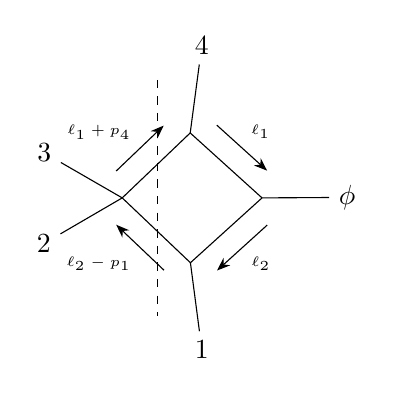
\begin{tikzpicture}[baseline=(current bounding box.center)]
 	 \begin{feynman}
    		\diagram [horizontal=b to d] {
      			a -- [momentum={\tiny\(\ell_2-p_1\)}] b
        			-- [momentum={\tiny\(\ell_1+p_4\)}] c
        			-- [momentum={\tiny\(\ell_1\)}] d -- [momentum={\tiny\(\ell_2\)}] a,
			d3  [particle=\(3\)]-- [] b,
			d2 [particle=\(2\)]-- [] b,
      			d1 [particle=\(1\)]-- [] a,
      			d4 [particle=\(4\)]-- [] c,
      			d -- [] s [particle=\(\phi\)],
   		 };
    		\coordinate (midpoint) at ($(b)!0.25!(d)$);
   		\draw [dashed] ($(midpoint) + (0, 1.5)$) -- ($(midpoint) + (0, -1.5)$);
  	\end{feynman}
	\end{tikzpicture}
	\right]&&+ C^B_{3,1} \left[
	\begin{tikzpicture}[baseline=(current bounding box.center)]
 	 \begin{feynman}
    		\diagram [horizontal=s to d] {
      			d2 [particle=\(\phi\)]-- b -- [momentum={\tiny\(\ell_2\)}] c
        			-- [momentum={\tiny\(\ell_1\)}] d -- [momentum={\tiny\(\ell_1-p_1\)}] b,
      			d1 [particle=\(2\)]-- [] b,
			d3  [particle=\(3\)]-- [] c,
      			d4 [particle=\(4\)]-- [] c,
      			d -- [] s [particle=\(1\)],
   		 };
    		\coordinate (midpoint2) at ($(b)!0.5!(d)$);
		\coordinate (midpoint) at ($(c)!0.5!(d)$);
   		\draw [dashed] ($(midpoint2) + (1.5, -0.15)$) to[out=180, in=90] ($(midpoint) + (-0.35, -1)$);
  	\end{feynman}
	\end{tikzpicture}\right]\\
	&&
	+ C^B_{3,2} \left[
	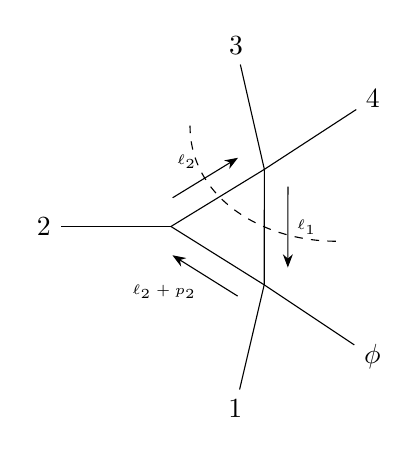
\begin{tikzpicture}[baseline=(current bounding box.center)]
 	 \begin{feynman}
    		\diagram [horizontal=s to d] {
      			d2 [particle=\(3\)]-- b -- [momentum={\tiny\(\ell_1\)}] c
        			-- [momentum={\tiny\(\ell_2+p_2\)}] d -- [momentum={\tiny\(\ell_2\)}] b,
      			d1 [particle=\(4\)]-- [] b,
			d3  [particle=\(\phi\)]-- [] c,
      			d4 [particle=\(1\)]-- [] c,
      			d -- [] s [particle=\(2\)],
   		 };
    		\coordinate (midpoint2) at ($(b)!0.5!(d)$);
		\coordinate (midpoint) at ($(c)!0.5!(d)$);
   		\draw [dashed] ($(midpoint2) + (1.5, -0.55)$) to[out=180, in=-90] ($(midpoint) + (-0.35, 1.65)$);
  	\end{feynman}
	\end{tikzpicture}\right]
 \end{eqnarray*}
\end{document}